%Section 3.1
\section{The LHC Machine}

The Large Hadron Collider (LHC)\cite{LHC}, located at the European Organization for Nuclear Research (CERN) complex in Geneva Switzerland, is the world's largest and most powerful particle collider as well as the most complex experimental device ever assembled. The main motivation for its construction was uncovering the nature behind electroweak symmetry breaking due to the Higgs mechanism as well as to search for new physical phenomena Beyond the Standard Model (BSM)\cite{BSM}. Since its completion in 2008, the LHC has helped researchers obtain a plethora of significant results in the field of particle physics and it successfully achieved its purpose with the discovery of the Higgs Boson in 2012.\\

The LHC consists of several superconducting magnets and accelerating structures arranged along a 27-kilometer circumference ring which serve to boost and bend the proton (or other heavy ion) beams along its path. In order for the particle beams to maintain the orbit while they are accelerated, a magnetic field of 8.3 T is produced by the superconducting magnets along the circular tunnel, 100 meters below the ground. The magnets are maintained at a temperature of 1.9 K by using liquid helium. The two beams are made to travel in opposite directions and in separate beam pipes which are kept at ultrahigh vacuum and are accelerated to near the speed of light. They are then collided head-on at any of the four interaction points located around the LHC ring. Approximately 1.5x$10^{11}$ protons are generated every 25 ns with an energy of 26 GeV at the Proton Synchrotron (PS). The proton beam is then accelerated to an energy of 450 GeV at the Super Proton Synchrotron (SPS)\cite{SPS} before being delivered to the LHC. At design level, each bunch is accelerated to an energy of 7 TeV and are made to collide at a centre-of-mass energy of up to 14 TeV with a frequency of 40 MHz.  The current proton beams achieve an instantaneous luminosity on the order of 10$^{32}$ cm$^{-2}\cdot$s${^{-1}}$ and a total integrated luminosity of 37 fb$^{-1}$ was reached during 2016\cite{CMSLHC}.\\

%\begin{comment} %
\begin{figure}[tb]
\begin{center}
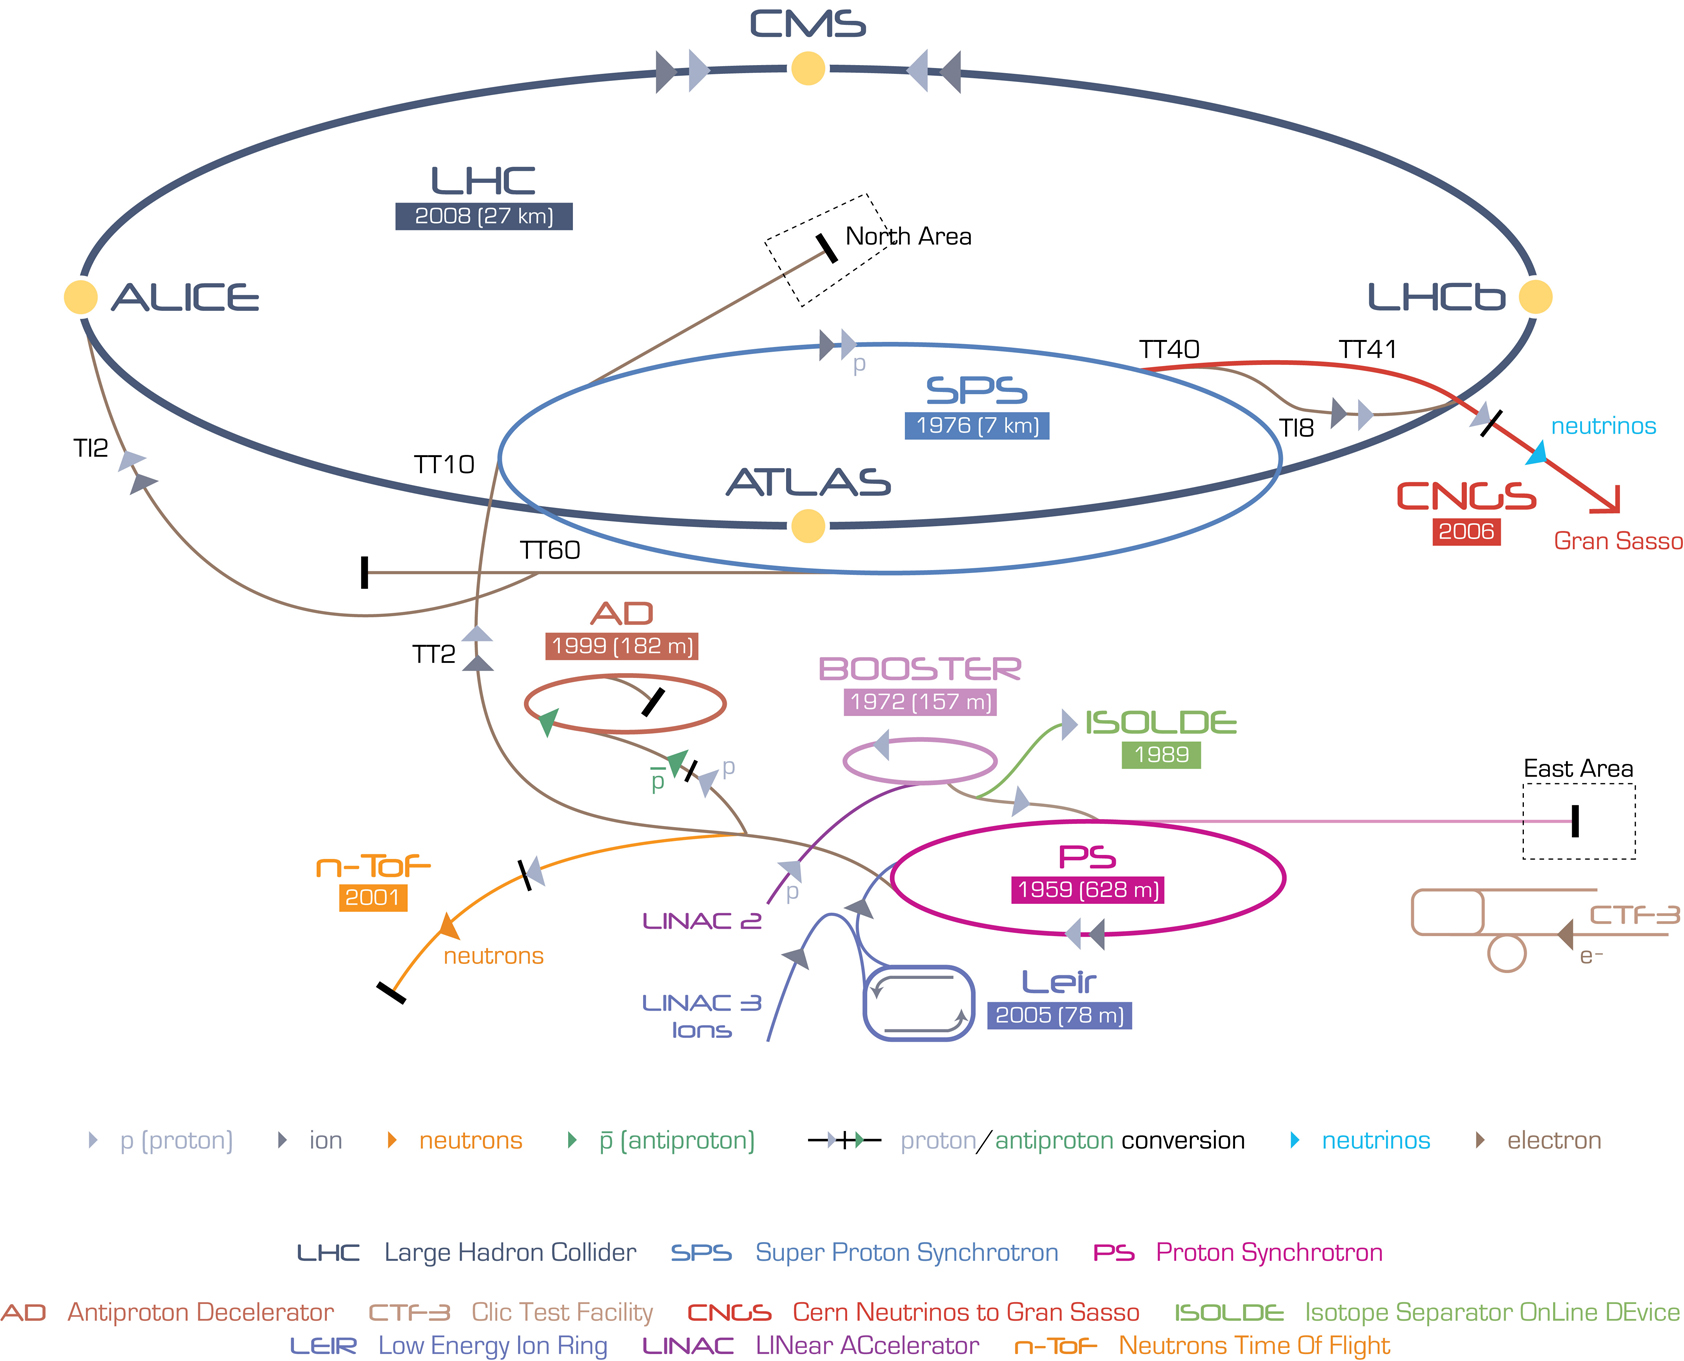
\includegraphics[width=1.0\textwidth]{Cern-Accelerator-Complex.jpg} 
\caption{The CERN Accelerator Complex\cite{LHCcomplex}.}
\label{Cern-Accelerator-Complex.jpg} 
\hspace{4em}
\end{center}
\end{figure}
%\end{comment} %

The four main detectors comprising the LHC machine are CMS, ATLAS\cite{ATLAS}, LHCb\cite{LHCb} and ALICE\cite{ALICE}. Both CMS and ATLAS are general purpose detectors whose initial designs had the detection of the SM Higgs boson, with its wide range of decay modes, in mind. Both detectors managed to accomplish this goal when a 126 GeV scalar boson consistent with the SM Higgs was independently verified by both experiments in July of 2012. Furthermore, the designs for CMS and ATLAS allow for the search of many other additional phenomena in BSM physics such as Supersymmetry, Dark Matter\cite{DM}, Dark Sector\cite{DS}, etc. On the other hand, the LHCb and ALICE detectors focus on more particular kinds of searches. The main motivation for the LHCb experiment, where the b stands for beauty, concerns itself with the measurement of CP violation parameters in b-hadron interactions and studies cover a wide range of aspects of Heavy Flavor Electroweak and QCD physics. Meanwhile, the ALICE experiment focuses on the study of heavy ion (Pb-Pb) nuclei collisions at a centre-of-mass energy of 2.76 TeV in order to better understand the physics behind strongly interacting matter at extreme energy densities.

%Section 3.2
\section{The CMS Detector}
The Compact Muon Solenoid (CMS) detector is a general purpose particle detector designed to investigate various physical phenomena concerning the SM and beyond it, such as Supersymmetry, Extra Dimensions and Dark Matter. As its name implies, the detector is a solenoid which is constructed around a superconducting magnet capable of producing a magnetic field of 3.8 T. The magnetic coil is 13m long with an inner diameter of 6m, making it the largest superconducting magnet ever constructed. The CMS detector itself is 21m long with a diameter of 15m and it has a weight of approximately 14,000 tonnes. The CMS experiment is one of the largest scientific collaborations in the history of mankind with over 4,000 participants from 42 countries and 182 institutions.\\

%\begin{comment} %
\begin{figure}[tb]
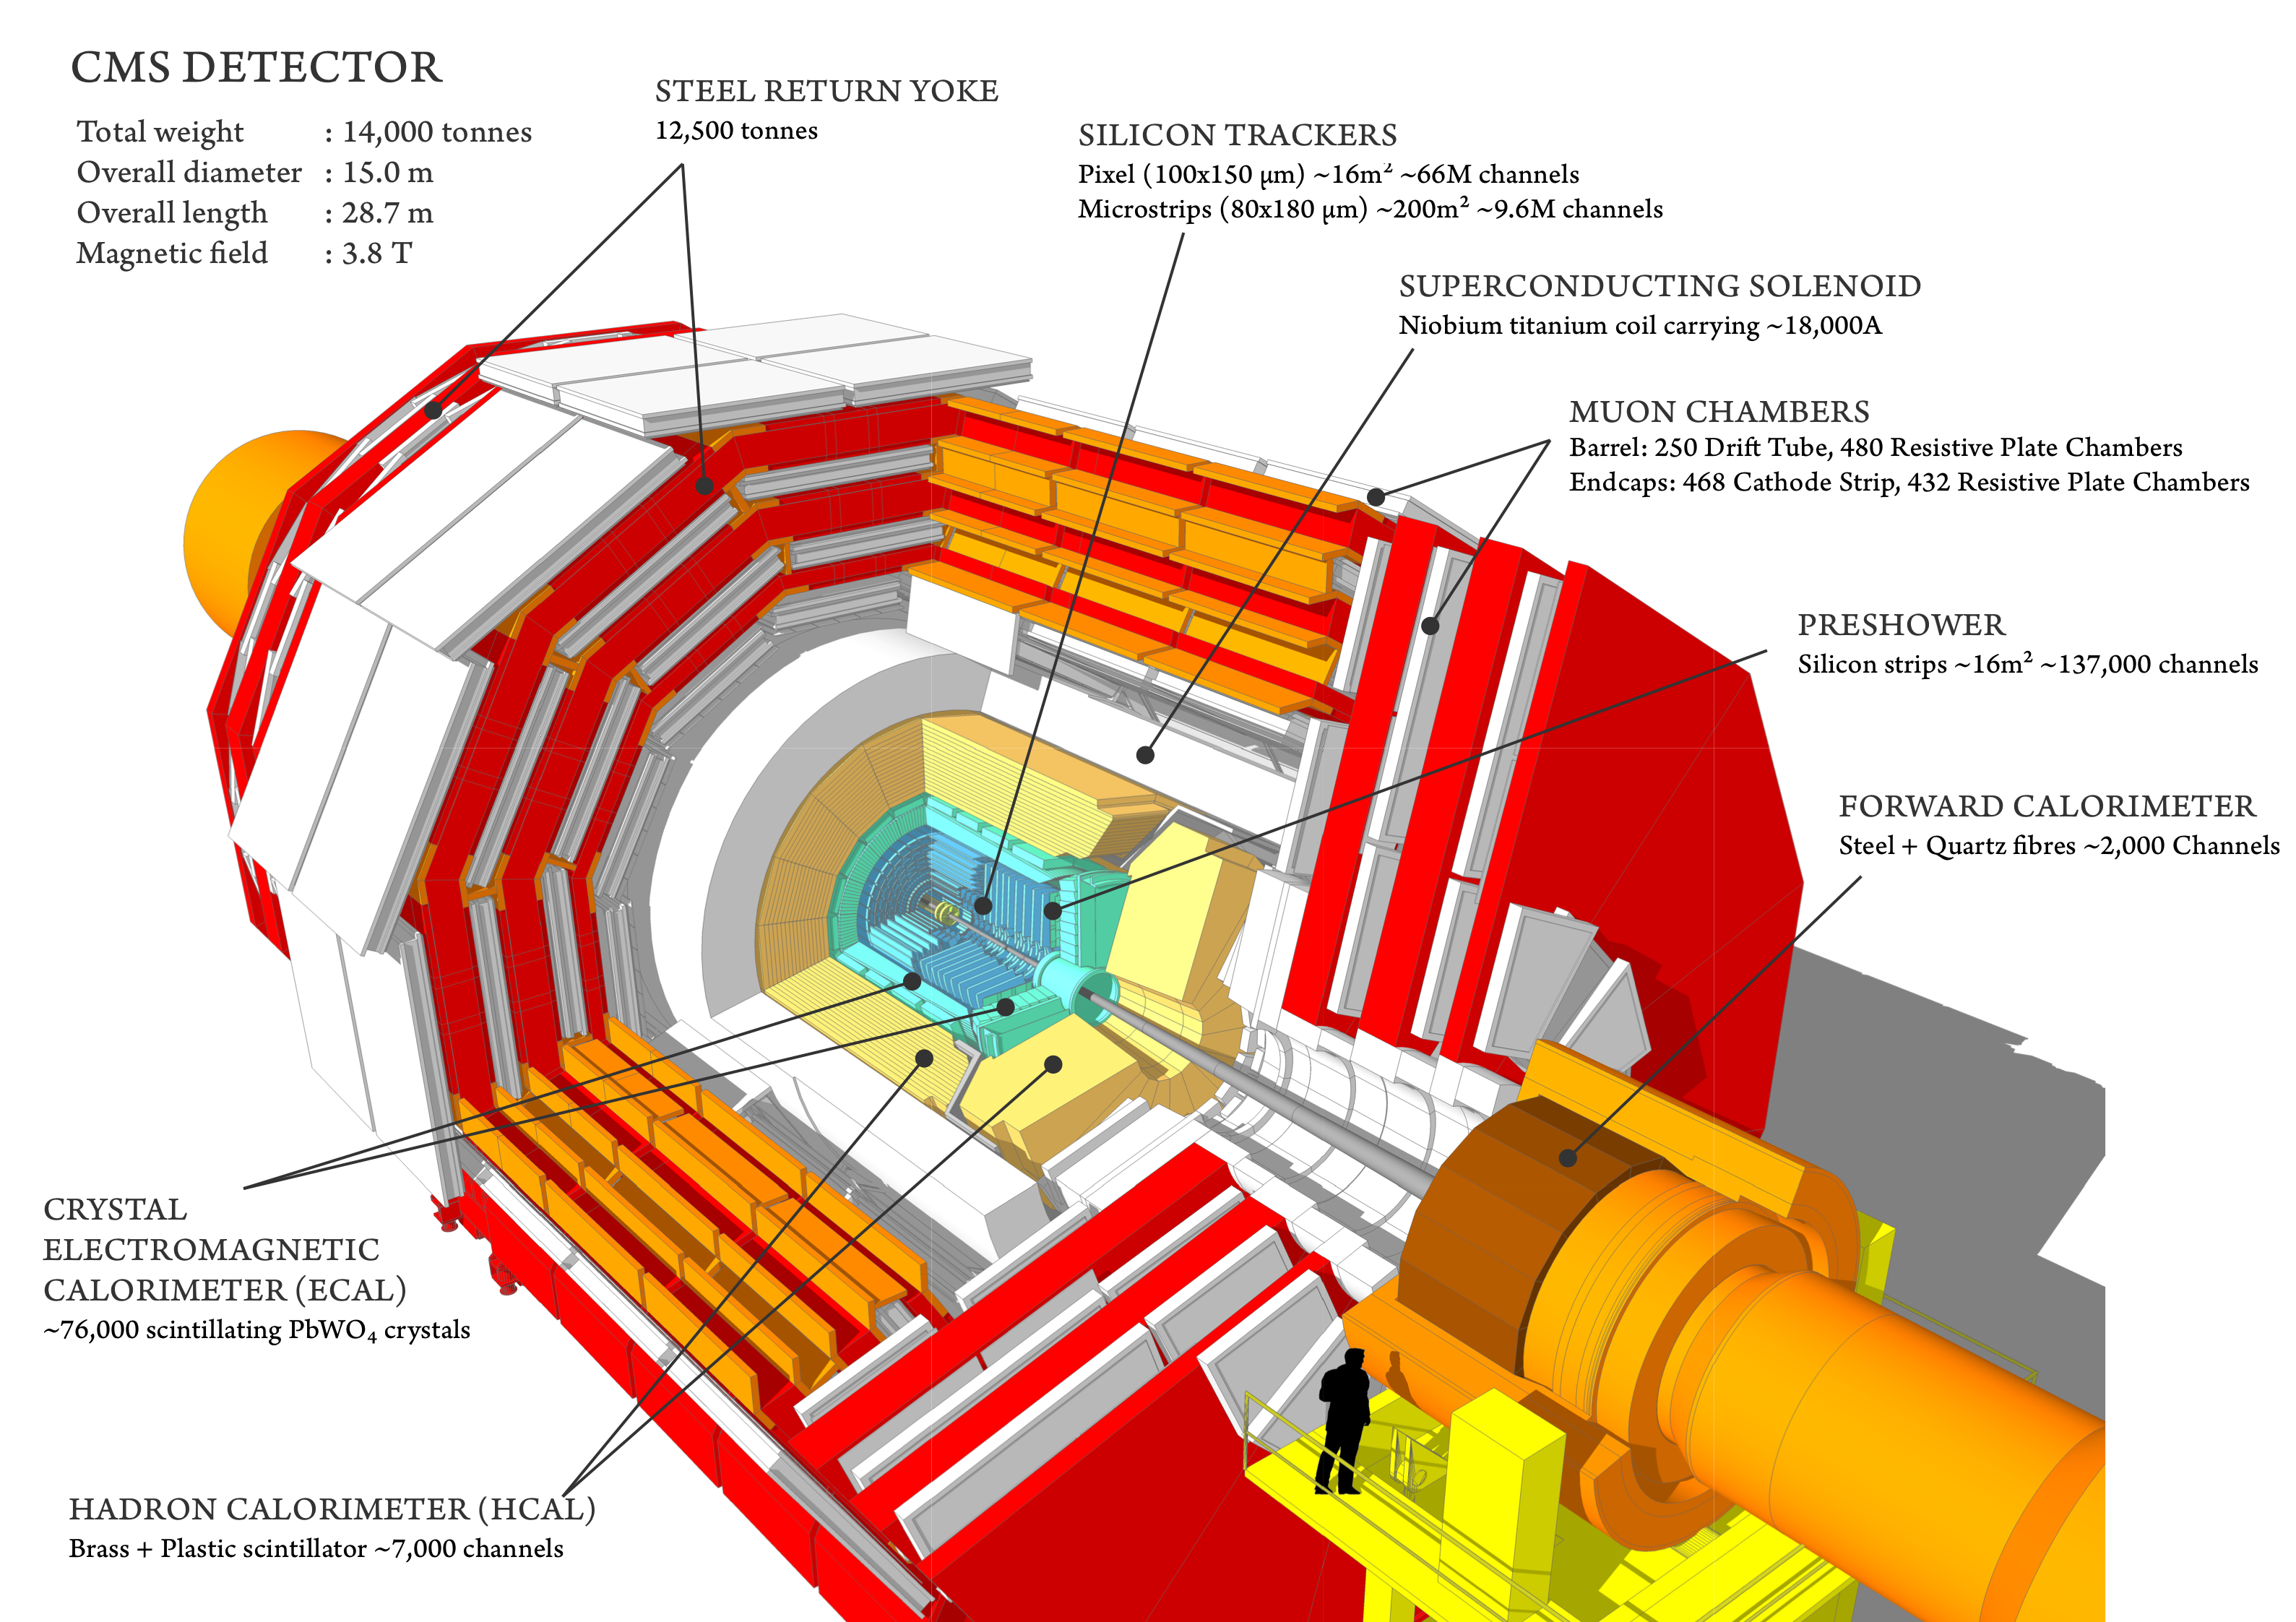
\includegraphics[width=1.0\textwidth]{CMSLayout.png} 
\caption{The CMS Detector Layout\cite{CMSlayout}.}
\label{CMSLayout} 
\hspace{4em}
\end{figure}
%\end{comment} %

In order to meet the many needs of the SM and BSM searches, and the goals of the LHC physics program, the CMS detector was designed with the following features:\\
\begin{itemize}
	\itemsep-1em
	\item{A magnet with large bending power and high performance muon detector for good muon identification and momentum resolution over a wide range of momenta and angles.}\\
	\item{An inner tracking system capable of high reconstruction efficiency and momentum resolution requiring pixel detectors close to the interaction region.}\\
	\item{An electromagnetic calorimeter able to provide good electromagnetic energy resolution and a high isolation efficiency for photons and leptons.}\\
	\item{A hadron calorimeter capable of providing precise missing-transverse-energy ($p_\text{T}^{miss}$)  and dijet-mass resolution.}\\
\end{itemize}

A general layout of the CMS detector and all its constituent sub-detectors can be seen in \autoref{CMSLayout}. The configuration of the CMS sub-detectors follow a cylindrical layer pattern that is symmetrical about the interaction region and consists of a central barrel with endcaps on both ends.

The coordinate system for the CMS detector design uses a right-hand rule convention centered around the ideal interaction point to describe the positions of objects in the experiment. The z-axis is defined along the direction of the LHC beam, with the x-axis pointing towards the center of the LHC ring. In terms of polar coordinates then, r is the radial distance from the center of the pipe, the polar angle $\theta$ is measured against the z-axis and the azimuthal angle $\phi$ is measured with respect to the x-axis. However, the pseudorapidity $\eta$ is generally preferred over the polar angle $\theta$. The pseudorapidity is defined as:

\begin{center}
$\eta$ =  $-$ ln tan $\frac{\theta}{2}$.
\end{center}

\subsection{Silicon Tracking System}

The CMS tracking system was designed with the goal of obtaining precise and efficient measurements for the trajectories of charged particles resulting from proton-proton collisions at the LHC. 
In addition, it allows for the precise measurement of secondary vertices and impact parameters needed to efficiently identify the heavy flavours produced in many interesting physics channels. Due to the LHC's design Luminosity of 10$^{34}$ cm$^{-2}$s$^{-1}$, the currently installed CMS phase-1 tracker is expected to handle an average of 1000 particles from over 20 overlapping proton-proton interactions per bunch crossing, every 25 ns. This required a detector technology capable of achieving a high granularity and fast response as well as being tolerant to the radiation produced from the intense particle flux. These considerations lead to a tracker design composed entirely of silicon detector technology which features an active silicon area of about 200 m$^2$, making it the largest silicon tracker ever built\cite{CMSdet1}.\\

%\begin{comment} %
\begin{figure}[tb]
\begin{center}
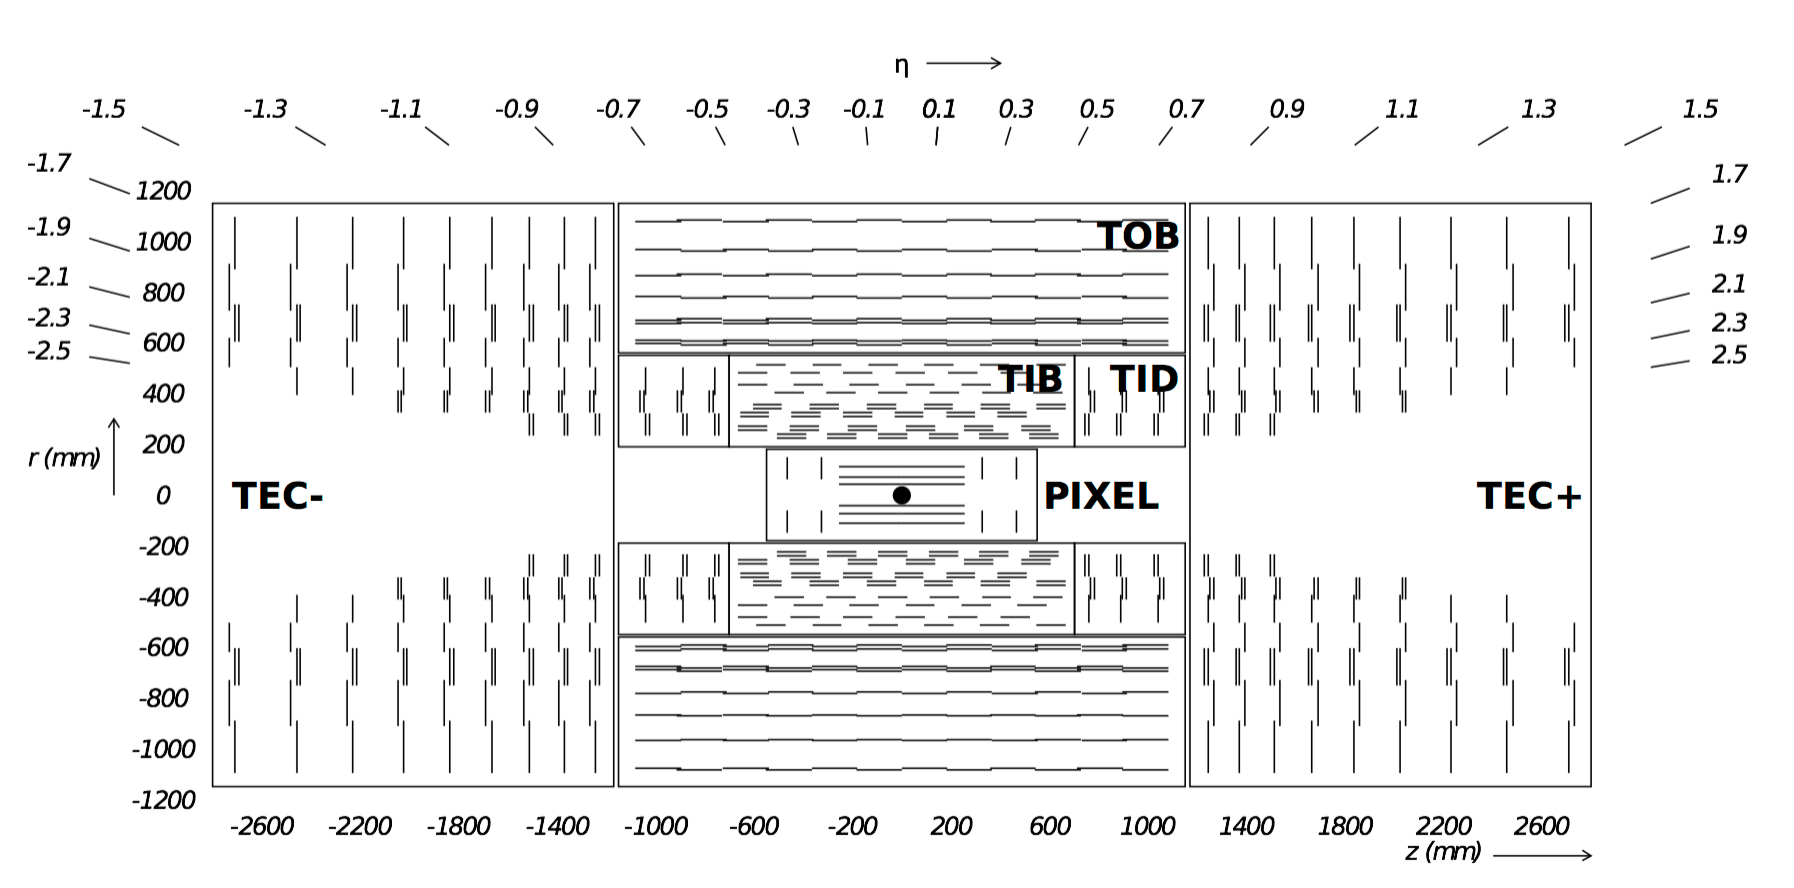
\includegraphics[width=0.9\textwidth]{CMSTrackerLayout.png} 
\caption{Overview of the CMS Tracker Layout\cite{CMSdet2}.}
\label{CMSTrackerLayout} 
%\hspace{4em}
\end{center}
\end{figure}
%\end{comment} %

The CMS tracker is built in a cylindrical manner around the interaction point and has a diameter of 2.5 m and a length of 5.8 m. It is comprised of a pixel detector with three barrel layers, positioned at a distance between 4.4 cm and 10.2 cm from the interaction region, and a silicon strip tracker with 10 barrel detection layers extending to a radius of 1.1 m. Each system is made complete by endcaps at opposite sides of the barrel, consisting of 2 discs for the pixel detector and 3 plus 9 discs for the strip tracker, extending the acceptance region of the tracker up to a pseudorapidity $|\eta| <$ 2.5.\\

The pixel detector is the part of the CMS tracking system closest to the interaction region and consists of 3 barrel layers (BPix) and 2 endcap discs (FPix). It is responsible for providing precise tracking points in $r$-$\phi$ and $z$, a feature that is required for the small impact parameter resolution, needed for good secondary vertex reconstruction. The detector contains 1440 modules covering an area of approximately 1 m$^2$ making up a total of 66 million pixels. The sensors were designed using an n-on-n concept from 320 $\mu$m thick silicon wafers and are fabricated with read-out chips (ROCs) that are bump-bonded to the sensor in standard 0.25 $\mu$m CMOS technology. Each of the pixels has a pitch size of 100 $\times$ 150 $\mu$m$^2$, which corresponds to an occupancy of about 10$^{-4}$ per bunch crossing.\\

The silicon strip tracker is built surrounding the pixel detector and consists of three large subsystems. The Tracker Inner Barrel and Disks (TIB/TID) extend to a radius of 55 cm and are composed of four barrel layers, completed by three disks at each end. The TIB/TID employs the use of 320 $\mu$m thick silicon micro-strip sensors in order to deliver up to 4 $r$-$\phi$ measurements on a trajectory. Surrounding the TIB/TID is the Tracker Outer Barrel (TOB), which consists of 6 barrel layers and has an outer radius of 116 cm. The TOB extends symmetrically in $z$ between $\pm$118 cm and provides an additional 6 $r$-$\phi$ measurements for a trajectory. Beyond the TOB's $z$ range lie the Tracker Endcaps (TEC+ and TEC-, where the sign indicates their position respect to $z$). Each TEC consists of 9 discs with up to 7 rings of silicon micro-strip detectors, providing up to 9 additional $\phi$ measurements per trajectory. The CMS silicon strip tracker has a total active silicon area of 198 m$^2$ and is composed of 15,148 sensor modules.

\subsection{Electromagnetic Calorimeter}
The CMS Electromagnetic Calorimeter (ECAL) is a hermetic homogeneous calorimeter whose function is to measure the energy of particles that interact via the electromagnetic force. With the use of 75,848 scintillator crystals, it is capable of providing good energy resolution within the requirements of the ambitious LHC program. In particular, the ECAL's design was optimized to search for diphoton events resulting from Higgs boson decays (H $\rightarrow \gamma \gamma$).\\ 

%\begin{comment} %
\begin{figure}[tb]
\begin{center}
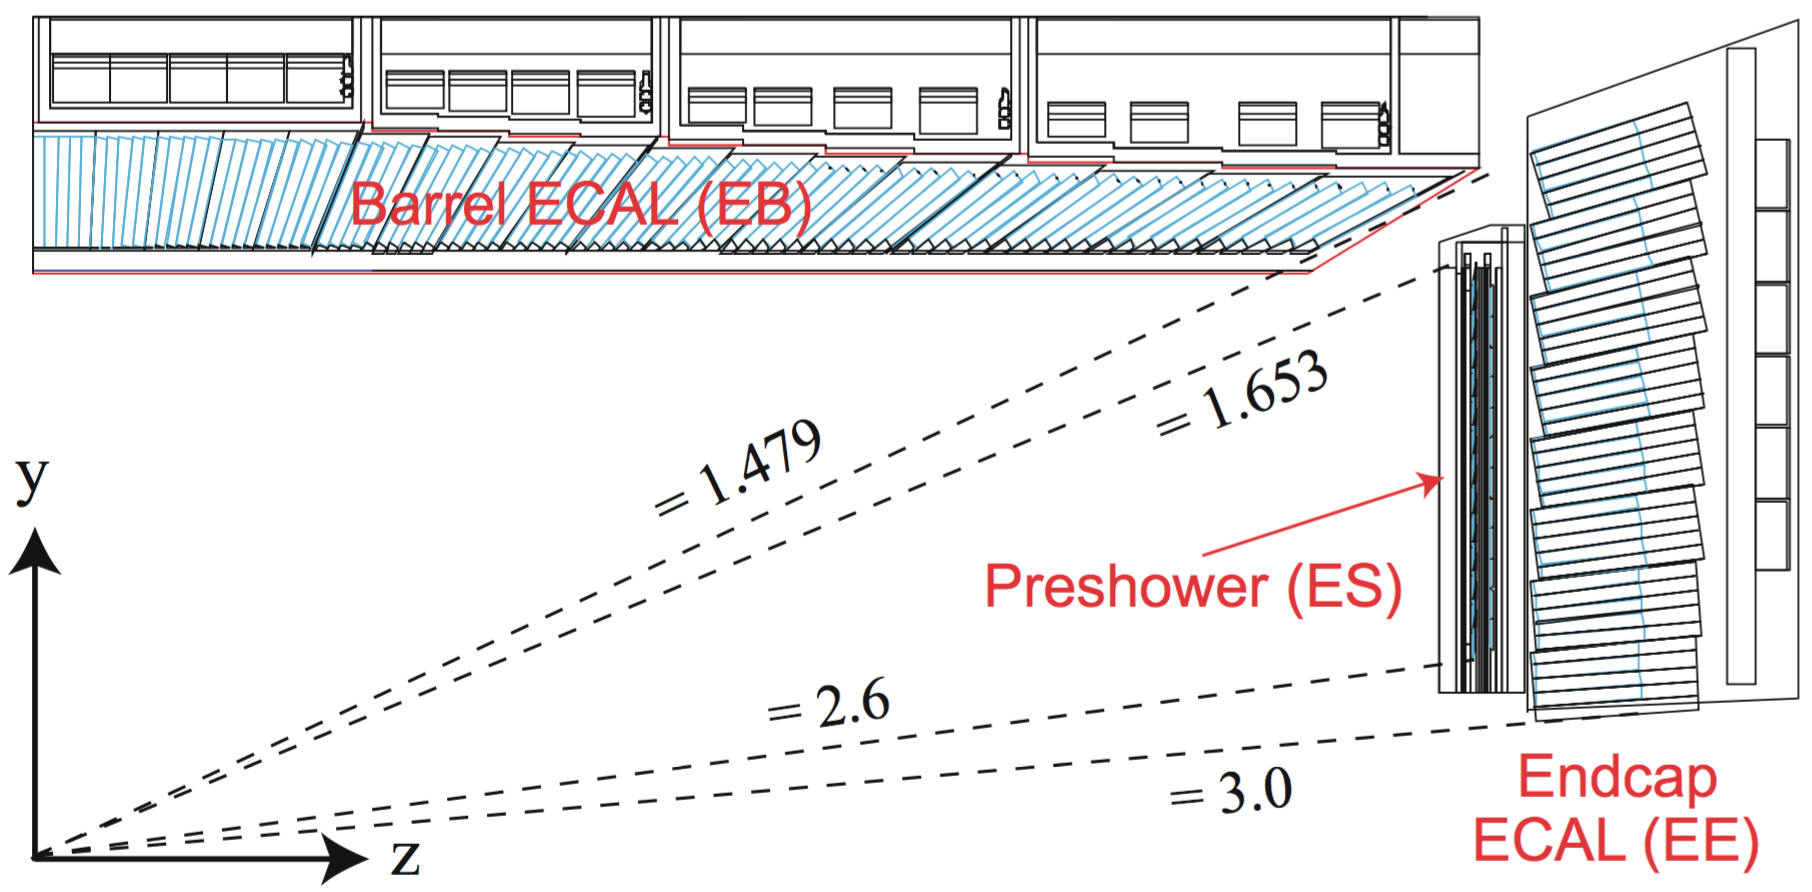
\includegraphics[width=0.8\textwidth]{ECALgeometry.png} 
\caption{Geometrical layout of the CMS Electromagnetic Calorimeter\cite{CMSLHC}.}
\label{CMS_ECAL_Geometry} 
\hspace{4em}
\end{center}
\end{figure}
%\end{comment} %

The ECAL is composed of two main sub-systems -- the barrel calorimeter (EB) and the endcap calorimeter (EE) -- and is completed by a preshower calorimeter (ES), as shown in \autoref{CMS_ECAL_Layout}. It covers a solid angle up to a pseudorapidity of $|\eta| <$ 3, with the EB extending in the range of $|\eta| <$ 1.479 and the EE covering a range of  1.479 $< |\eta| <$ 3. Both subsystems are composed of lead tungstate (PbWO$_4$) scintillator crystals which provide a fast response time and high radiation tolerance, both crucial requirements for optimal performance at LHC operating conditions. In addition, the properties of the PbWO$_4$ crystals (high density, short radiation and small Moli\'ere radius) led to the design of a compact calorimeter with fine granularity.\\

The barrel part of the ECAL (EB) is composed of specially designed avalanche photodiodes (APD). It consists of 61,200 crystals, forming a total volume of 8.14 m$^3$ and weighing about 67.4 t. The crystals that form the EB are 230 mm long with a cross-section of 22$\times$22 mm$^2$ at the front face and 26$\times$26 mm$^2$ at the back. They are organized in pairs within thin-walled alveolar structures called submodules. The submodules are assembled into different types of modules that differ by their location with respect to $\eta$ and contain 400 or 500 crystals each. Theses modules are then arranged in sets of four modules, called supermodules, and contain 1700 crystals each. Thus, the EB is composed of two half-barrels, each consisting of 18 supermodules.\\

In contrast, the photodetectors used in the endcap section of the ECAL are vacuum phototriodes (VPT)\cite{VPT}. Each of the endcaps contain 7,324 crystals which, in total, occupy a volume of 2.90 m$^3$ and weigh about 24.0 t. The crystals in the EE are 220 mm in length with a cross-section of 28.62$\times$28.62 mm$^2$ for the front face and 30$\times$30 mm$^2$ in the rear. They are all identical in shape and are arranged in mechanical units of 5$\times$5 crystals, called supercrystals (SC), which consist of carbon-fibre alveola structures. Each of the endcaps are divided into two semi-circular structures, called \textit{Dees}, which hold a total of 3,662 crystals. \\

The ES preshower is located before the EE detector and spans a pseudorapidity range of 1.653 $< |\eta| <$ 2.6. It's main purpose is to identify neutral pions in the endcaps as well as to improve the determination of electrons and photons with high granularity. The preshower consists of two layers and has a total thickness of 20 cm. The first layer is conformed by lead radiators which initiate electromagnetic showers from incoming photons and electrons. Meanwhile, the second layer is composed of silicon strips which are capable of measuring the deposited energy and the transverse shower profiles.

%\begin{comment} %
\begin{figure}[tb]
\begin{center}
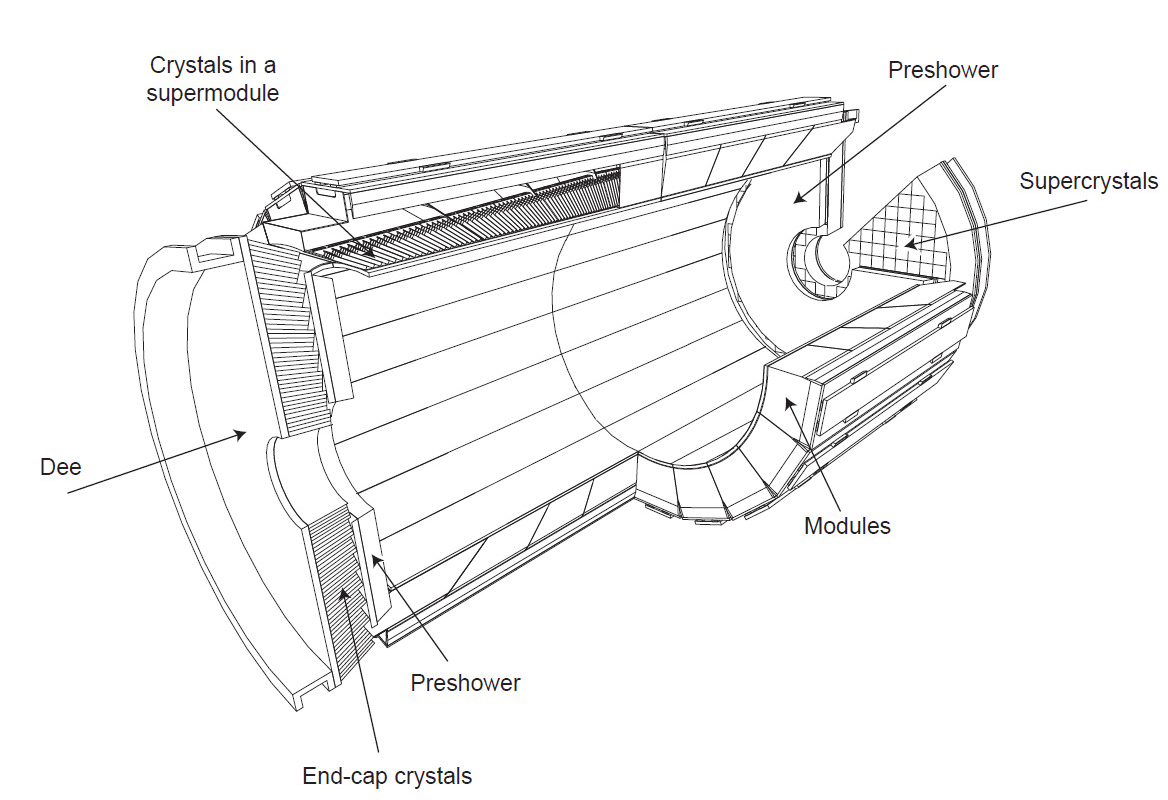
\includegraphics[width=0.9\textwidth]{ECALlayout.png} 
\caption{Layout of the CMS ECAL illustrating its various components\cite{CMSdet1}.}
\label{CMS_ECAL_Layout}
\vspace{-1em}
\end{center}
\end{figure}
%\end{comment} %

\subsection{Hadron Calorimeter}

The CMS Hadron calorimeter (HCAL) conforms the next layer of the CMS detector. It is a sampling calorimeter that consists of alternating layers of massive absorbing brass plates and plastic scintillator tiles and is of particular importance for the measurement of hadron jet energy and  $p_\text{T}^{miss}$. The HCAL detector is located in between the outer extent of the ECAL ($R$ = 1.77 m) and the inner extent of the magnet coil ($R$ = 2.95 m). Similar to the other CMS subsystems, it's composed of a barrel part (HB) and an endcap part (HE). In addition, it features a tail-catching outer calorimeter (HO), located outside the magnet, and a forward calorimeter (HF) in the very forward region near the beam line. A layout of the HCAL system can be seen in \autoref{CMS_HCAL_Layout}.\\

%\begin{comment} %
\begin{figure}[tb]
\begin{center}
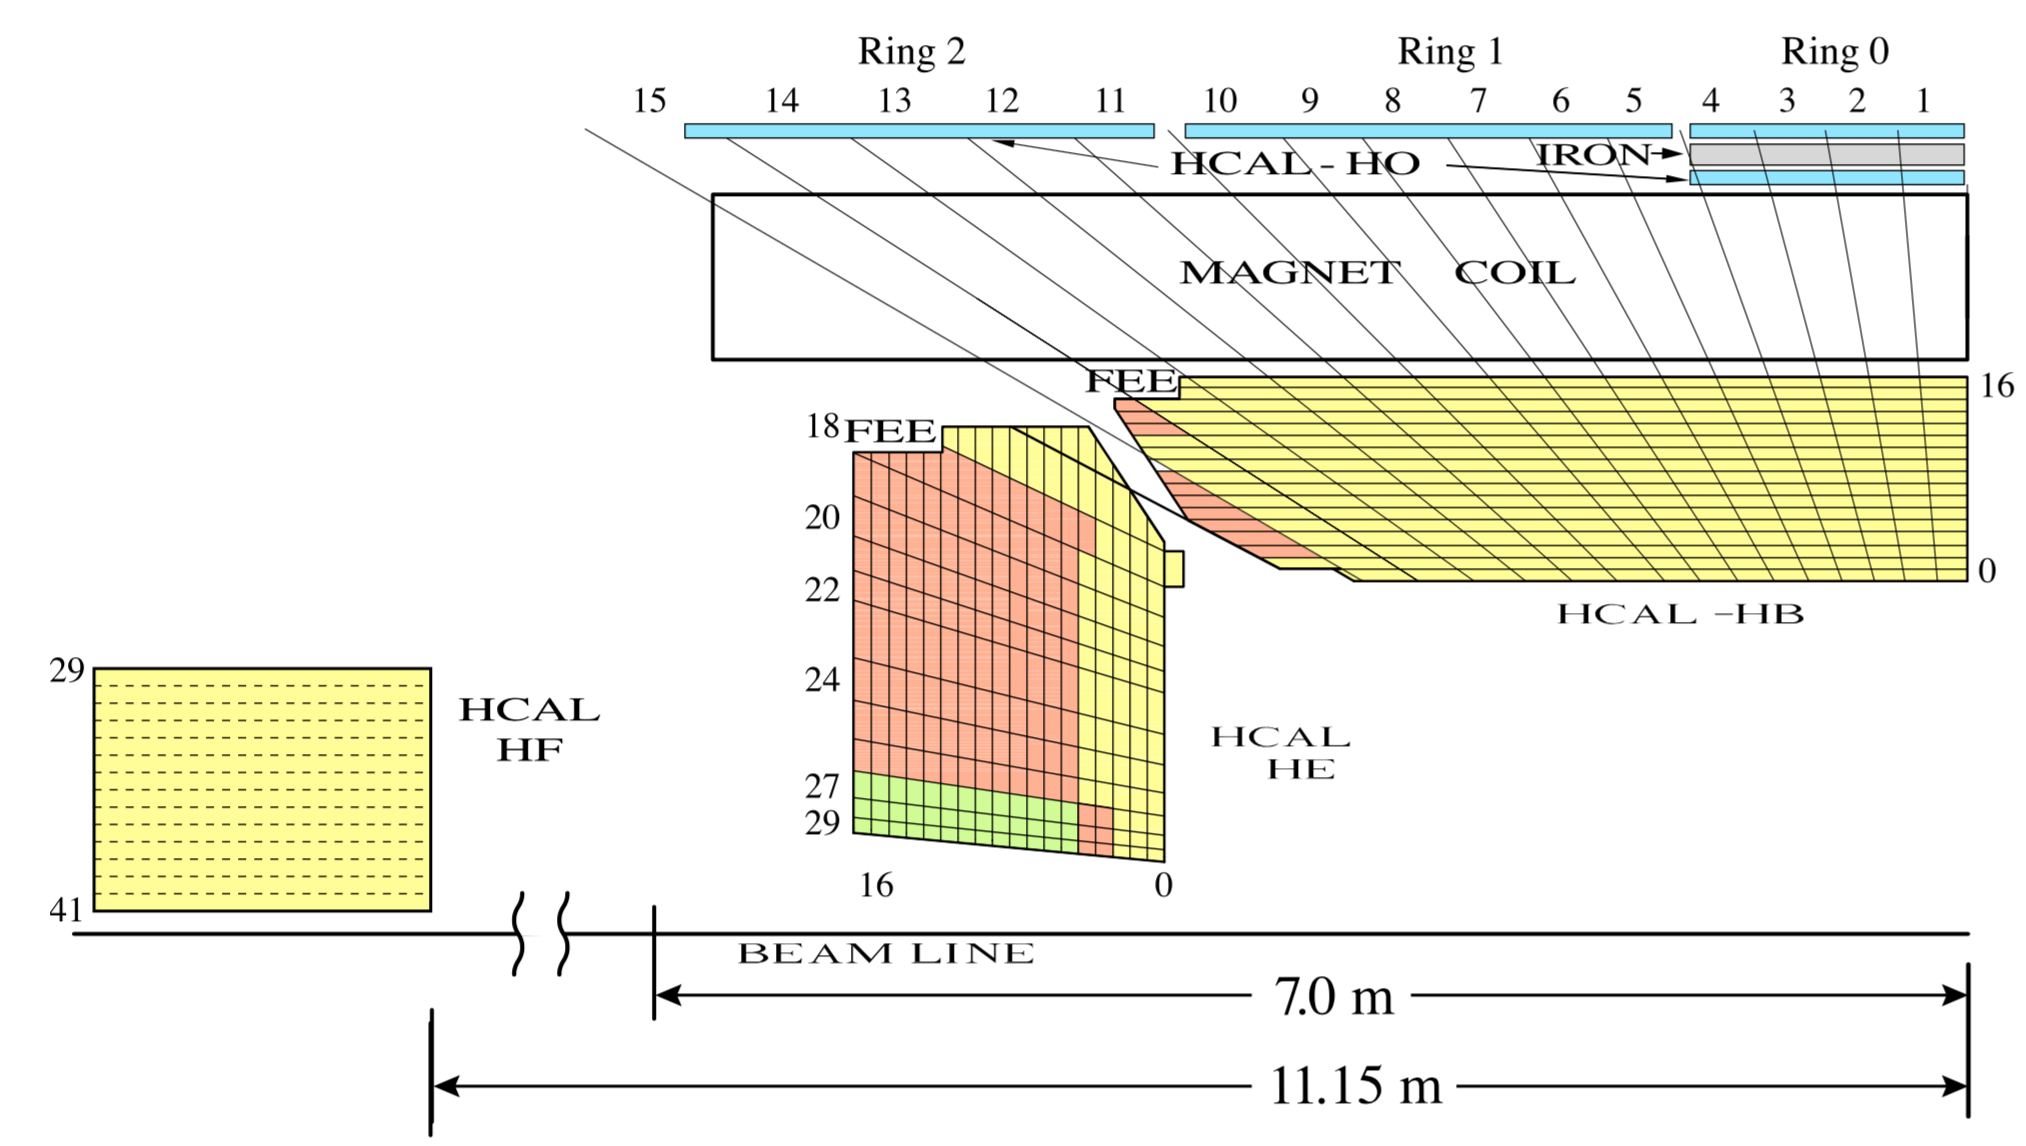
\includegraphics[width=0.9\textwidth]{CMS_HCAL.png} 
\caption{Geometrical layout of the HCAL showing the locations of the hadron barrel (HB), endcap (HE), outer (HO) and forward (HF) calorimeters\cite{CMShcal}.}
\label{CMS_HCAL_Layout} 
\end{center}
\end{figure}
%\end{comment} %

The barrel component of the HCAL is a sampling calorimeter which covers the pseudorapidity range $|\eta|<$1.3. It consists of both the HB and the HO detectors. The reason behind separating the barrel detector into the HB and HO is due to the limited amount of space available for the barrel detector. The HB is located within the superconducting magnet coil and is supplemented by the HO in between the outer solenoid coil and the muon chambers. Therefore, the HO acts as a tail-catcher in order to improve the jet energy measurements and $p_\text{T}^{miss}$, with the solenoid in between acting as absorber material. The HB consists of two half-barrel sections, identified as HB+ and HB- due to their geometrical location, which are composed of 36 identical azimuthal wedges. The wedges, which are constructed out of flat brass absorber plates, are aligned parallel to the beam axis and are segmented into four azimuthal angle ($\phi$) sections.\\ 

The HE covers a significant amount of the pseudorapidity in the range of 1.3 $< |\eta| <$ 3, a region containing about 34\% of the particles produced in the final state. Due to the high luminosity of the LHC, the HE is required to have a high radiation tolerance at $|\eta| \simeq 3$, as well as being capable of handling high counting rates. Similar to the HB, the HE is also composed of brass absorber plates and scintillator plates which are read out by wavelength shifting fibers. The light captured by the scintillators merges within the wavelength shifting fibers and then it's read out by hybrid photo-diodes. The scintillators are partitioned in towers with an area of $\Delta\eta\times\Delta\phi = 0.17\times0.17$.\\

\subsection{Magnet}

The CMS superconducting solenoid is one of the driving features of the detector design. It is capable of providing a magnetic field with a 3.8T magnitude, which allows for the large bending power needed for  precise particle transverse momentum ($p_{\text{T}}$) measurements. The magnet is made of four layers of stabilized reinforced Niobium-Titanium (NbTi) and has a cold mass of 220 t. The solenoid consists of a 13 m long coil with an internal diameter of 6 m, which houses both the tracking and calorimetric system. This design allows for particles to be measured prior to crossing the magnetic coil which significantly improves the energy resolution. 

\subsection{Muon Detector}

 As implied by the detector's name, precise and robust muon measurements have been a central theme of the CMS experiment since the early stages of its design. The detector design takes into account that muons behave as minimum ionizing particles (MIPs)\cite{MIPs} and can therefore manage to traverse
the tracker and calorimeters with minimal energy loss. Furthermore, due to their relatively long lifetime they can be efficiently identified by a dedicated system at the outer region of the detector. Consequently, the CMS muon systems comprise the outermost layer of the detector, which are integrated into the magnet return yoke that surrounds the solenoid.\\

The muon system is capable of three main functions: muon identification, muon $p_{\text{T}}$ measurement and triggering. It is composed of three different types of detectors, all of which make use of gaseous chamber technology. This choice of detector provides a cost efficient way of covering most of the full solid angle, featuring a total of 25,000 m$^2$ of detection plates. As a consequence of the shape of the solenoid magnet, the muon detector was designed to have a cylindrical barrel section as well as two planar endcap regions.\\

\begin{figure}[H]
\begin{center}
\begin{minipage}[b]{0.59\textwidth}
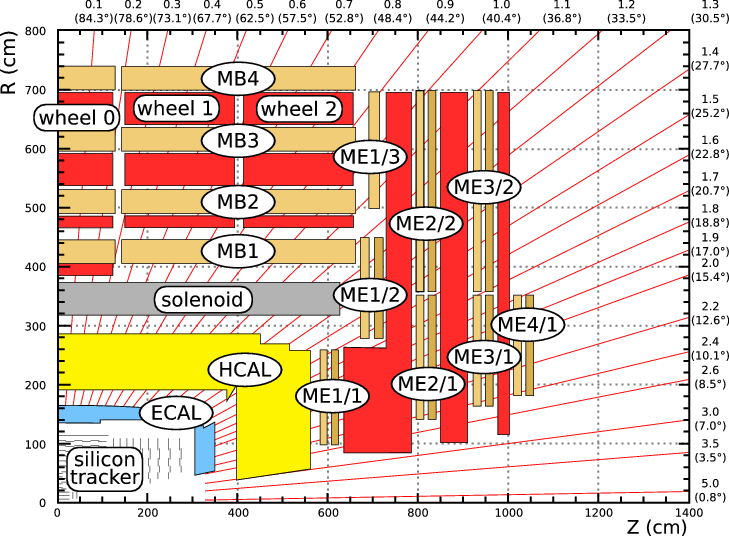
\includegraphics[width=\textwidth]{muonAlignment.png}
\end{minipage}
\hspace{1em}
\begin{minipage}[b]{0.3\textwidth}
    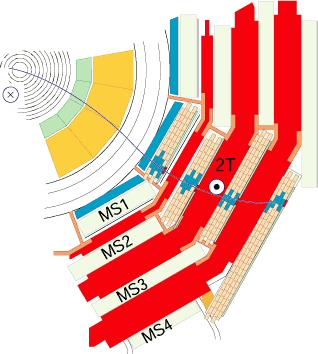
\includegraphics[width=\textwidth]{MuStations.png}
\end{minipage}
\end{center}
\vspace{-1em}
\caption[Quarter-view of the CMS muon system (left) and a muon in the transverse plane leaves a curved trajectory across the four muon detector stations (right).]{The left diagram shows a quarter-view of CMS with both the muon barrel (MB) and endcap (ME) stations \cite{muonAlignment}.  The right diagram shows a muon in the transverse plane leaves a curved trajectory across the four muon detector stations\cite{MuDet}.}
\label{muonSystem}
\end{figure}

For the barrel region of the muon detector, four layers of drift tube (DT) modules are used, covering a pseudorapidity of up to $|\eta| < 1.2$. These four layers, called ``stations'', are arranged in cylindrical concentric layers around the beam line, where the first three layers have 60 DTs each and the outer cylinder has 70. Each of the DT stations contain 12 individual gas filled tubes, all of which have a 4cm diameter and a center electrode. The use of DTs as tracking detectors for the barrel muon system is possible because of the low expected muon rate and the relatively low strength of the local magnetic field.\\
 
The endcap regions of the muon system are subject to a higher muon rate, and cover the range $0.9 < |\eta| < 2.4$ where the magnetic field is stronger and less homogeneous. Considering these conditions, cathode strip chambers (CSCs) are employed, which feature high granularity, fast response time and adequate radiation hardness. CSCs consist of arrays of positively-charged ``anode'' wires crossed with negatively-charged copper ``cathode'' strips within a gas volume. They are trapezoidal in shape and can cover either $\ang{10}$ or $\ang{20}$ in $\phi$. Furthermore, CSCs have the advantage of featuring both precision muon measurement and muon trigger in a single device.\\

The third type of detector used in the CMS muon system are called resistive plate chambers (RPCs) and can be found in both the barrel and endcap regions. They consist of gaseous parallel-plate detectors capable of providing precise timing information and adequate spatial resolution. Because of their excellent time resolution, RPCs provide the capability of tagging the time of an ionizing event between 2 consecutive LHC bunch crossings (BX) in a much shorter time ($\sim$ 1 ns) than the interval between the BXs (25 ns). For this reason, an RPC-based dedicated muon trigger device can be implemented to unambiguously identify the relevant BX to which a muon track is associated with, despite the high rate of events and background expected at the LHC.

\subsection{Trigger and Data Acquisition}

Due to the vast volume of data originating from the proton-proton collisions (delivered by the LHC at a rate of 40 MHz), a method of eliminating the majority of the uninteresting/unwanted events was a requisite for the CMS detector design. This event rate reduction is achieved by the implementation of the so-called trigger system, which manages to select the potentially interesting interactions and reduce the rate from a staggering 40 TBs$^{-1}$ to a manageable value of just a few hundred Hz.\\

The CMS trigger system is implemented using a two-stage rate reduction, which combines both a hardware and software phase. The combination of both of these triggers is designed to reduce the rate by a factor of $\sim10^6$. The first stage used in the rate reduction is purely hardware based and it is called the Level 1 (L1) Trigger \cite{L1T}, which consists of both Field Programmable Gate Array (FPGA) and Application Specific Integrated Circuit (ASIC) technology. During this initial stage, the rate is reduced to about 100 kHz with a latency of 3.2 ${\mu}$s. This time interval constrains the trigger decision, allowing only for data from the calorimeters and muon system to be processed. Trigger primitives (TP) from these subsystems are processed through a series of steps before the combined event information is evaluated by the global trigger (GT) where the final decision, whether or not to accept the event, is made.\\

The second stage, which implements offline-quality reconstruction algorithms in its event selection, is referred to as the High-Level Trigger (HLT)\cite{HLT}. The event selection process for the HLT requires that physics objects for each event, such as electrons, muons and jets, are reconstructed and undergo predetermined identification criteria. 

\subsection{Event Reconstruction}

In order to reconstruct the events the particle flow (PF) algorithm\cite{PFref} is used. This algorithm gathers information from all the CMS sub-detectors to reconstruct charged and neutral hadrons, photons, muons, and electrons. It relies on an efficient and pure track reconstruction, a clustering algorithm able to distinguish overlapping tracks originated from different vertices, and an efficient link procedure to associate each particle deposit in the sub-detectors. Once all the deposits of a particle are associated, it can be correctly identified and its four-momentum optimally determined from the combined information of the sub-detectors. The resulting list of particles are then used to reconstruct higher level objects such as jets, taus, missing transverse energy, and to compute charged lepton and photon isolation, etc\cite{Reco1}. The CMS experiment is provided with millions of collisions per second, which need to be triggered, detected, stored and analyzed in a collaboration of several thousand physicists. This huge amount of data and the complexity of the detector require a flexible data model that serves all the needs of the collaboration. The data format is optimized for performance and flexibility of the reconstruction for the end user's analysis.\\

\begin{figure}[tb]
\begin{center}
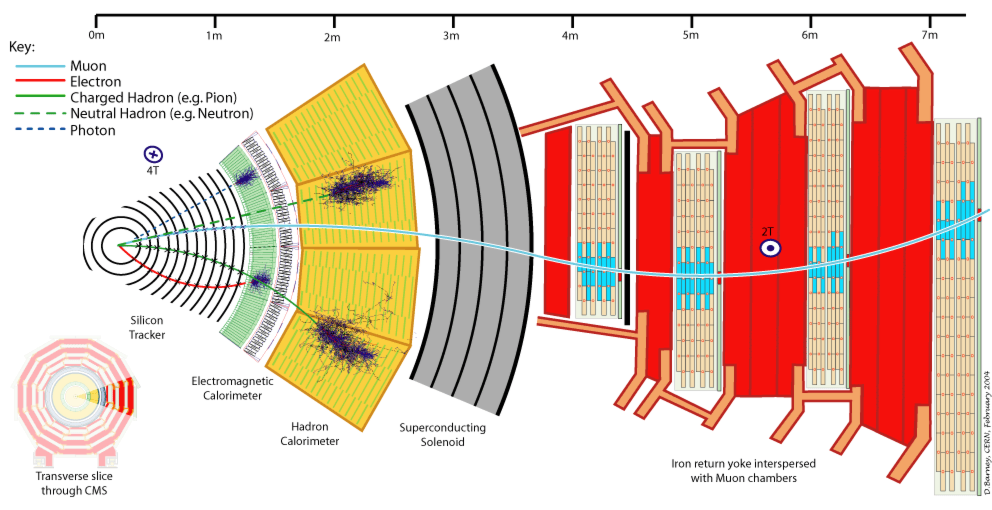
\includegraphics[width=1.0\textwidth]{CMSParticleDet.png} 
\caption{Transverse slice of the CMS detector, showing the individual detector subsystems and particle signatures in each. The particle type can be inferred by combining the detector response in the different subdetectors\cite{CMSslice}.}
\label{CMSParticleDet} 
\end{center}
\end{figure}

Event information from each step in the simulation and reconstruction chain is logically grouped into what is called a data tier\cite{CMScomp1}. From the physicist's point of view the most important data tiers are RECO, which contains all reconstructed objects and hits, and AOD (a subset of RECO). The AOD will contain a copy of all the high-level physics objects (such as muons, electrons, taus, etc.) and enough information about the event to support all the typical usage patterns of a physics analysis. It also contains a summary of the RECO information sufficient to support typical analysis actions such as track refitting with improved alignment or kinematic constraints, re-evaluation of energy and/or position of ECAL clusters based on analysis-specific corrections. The format of each data tier is ROOT \cite{ROOT}. ROOT is a framework for data processing developed at CERN with the sole purpose of aiding high energy physics research. The various AOD datasets are stored worldwide at various data tier centers. From the AOD's the analysis groups create data structures called NTuples containing only the high-level physics objects needed for their particular analysis. 

\subsection{Future Upgrade of Pixel Detector}
After the first LHC shutdown called LS1 (2013-2014), and the installation of the Phase-1 Pixel Detector \cite{Phase1FPix} in early 2017, among other things, the LHC is planning another series of upgrades during two major shutdowns, called LS2 and LS3, currently planned for 2019-2020 and $\sim$ 2024, respectively. LS2 would result in a further increase of the luminosity beyond the original design value, to over $2\cdot{10}^{34}$ cm$^{-2}$ s$^{-1}$.  With the LS3 upgrade of the LHC (called HL-LHC\cite{HLLHC}) the luminosity is expected to reach up to $7.5\cdot{10}^{34}$ cm$^{-2}$ s$^{-1}$. Correspondingly, the CMS collaboration has planned a series of further upgrades \cite{CMSPhase2,CMSupgrades} that will ensure the capabilities of the CMS detector to match to the HL-LHC running conditions, while taking the opportunity to improve the performance and repair any problems uncovered during the data-taking periods. The UPRM group will continue its involvement in the Phase-1 Pixel Detector operations and Phase-2 Pixel Upgrade design.\\

The HL-LHC conditions of instantaneous peak luminosities of up to $7.5\cdot{10}{^34}$ cm$^{-2}$ s$^{-1}$ and an integrated luminosity of the order of 300 fb$^{-1}$ would result in 1 MeV neutron equivalent fluence of $2.3\cdot{10}^{16}$ neq/cm$^2$ and a total ionizing dose (TID) of 12MGy (1.2 Grad) at the center of CMS, where its innermost component, the Phase-2 Pixel Detector will be installed. The detector should be able to withstand the above radiation dose, handle projected hit rates of 3GHz/cm$^2$ at the lowest radius, be able to separate and identify particles in extremely dense collision debris, deal with a pileup of 140-200 collisions per bunch crossing and have a high impact parameter resolution. This translates into requiring a detector design that is highly granular, has thinner sensors and smaller pixels, and faster, radiation hard electronics compared to its Phase-1 counterpart. The selection of interesting physics events at the Level-1 (L1) trigger and inefficiency of selection algorithms in high pileup conditions further require the Tracker to be included in this trigger stage, helping reduce the event rate from 40 MHz rate to 7.5 kHz. The physics goals also require an increase in Pixel Detector coverage to $|\eta| = 4.0$ which improves the $p_{\text{T}}^{miss}$ resolution and particle-flow event reconstruction by providing $p_\text{T}$ measurements and trajectories for charged particles entering the calorimeters. The $p_{\text{T}}^{miss}$ resolution is an essential performance parameter for many BSM physics searches including SUSY and extra dimension models where particles escape undetected from the detector space. The smaller pixel size will further improve b-tagging as well as hadronic reconstruction and track reconstruction efficiencies within boosted jets, which can be produced from new heavy objects decaying to Higgs, Z bosons, or top quarks -- all heavy probes that can be exploited for new physics searches. Improving the b-tagging capabilities directly affects our analysis due to the importance of properly identifying top quark decays.\\

\begin{figure}[H]
\begin{center}
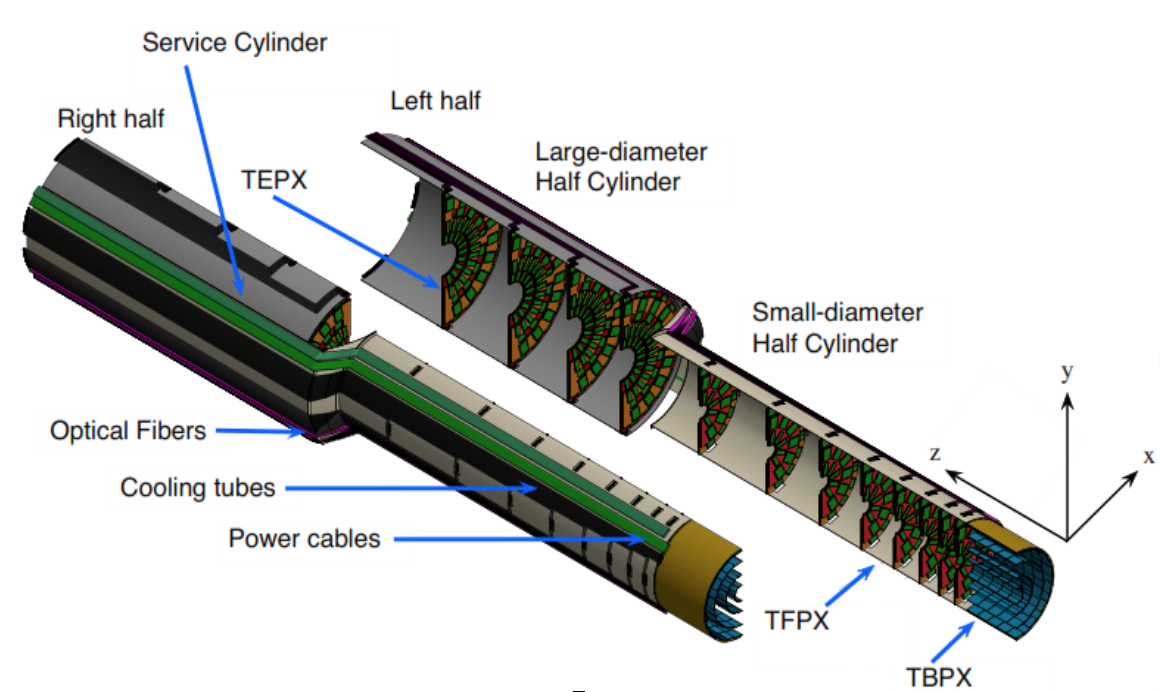
\includegraphics[width=0.8\textwidth]{PixelDet.png} 
\caption{Phase-2 Pixel Detector Layout[ref].}
\label{PixelDet} 
\end{center}
\end{figure}

The Phase-2 Pixel Detector\cite{Phase2Tracker,Phase2Tracker2} baseline design comprises a barrel part with 4 layers of Tracker Barrel Pixel Detector (TBPX), 8 small double-discs per side of Tracker Forward Pixel Detector (TFPX) and 4 large double-discs per side of Tracker Endcap Pixel Detector (TEPX). This forward and end part is referred to as 8l4s (8 TFPX and 4 TEPX). In the TBPX the pixel modules are arranged in ``ladders''. In each layer, neighboring ladders are mounted staggered in radius, so that $r$-$\phi$ overlap between the ladders is achieved. The modules on a ladder do not overlap in $z$. A projective gap at $\eta = 0$ is avoided by mounting an odd number of modules along $z$, and by splitting the barrel mechanics in $z$ into slightly asymmetric halves. In TFPX and TEPX the modules are arranged in concentric rings. Each double-disc is physically made of two discs, which facilitates to mount modules onto four planes, with overlaps in $r$ as well as $r$-$\phi$. Each disc is split into two halves, and these D-shaped structures are referred to as ``dees''. The TEPX will provide the required luminosity measurement capability, by an appropriate implementation of the readout architecture. In total, the pixel detector will have an active surface of approximately 4.9 m$^2$. \autoref{PixelDet} shows the layout of the Phase-2 Pixel Detector.





